% Root file

%%===================================
\documentclass[12pt]{report}
\usepackage{ramsstyle}
\usepackage{titlesec}
\usepackage{subcaption}
\usepackage{caption}
\usepackage{longtable}
\titleformat{\chapter}{\huge}{\thechapter.}{20pt}{\huge}
%%===================================
%Write the various parts of your thesis as separate files and include them into the main file by the command \include{name of included file}. When you compile the LaTeX file, you may choose which subfiles to include by the command

%\includeonly{chapter01,chapter02}

%%===================================
\begin{document}

%This is the Titlepage
%%=========================================
\thispagestyle{empty}

\includegraphics[scale=0.4]{Pictures/ntnu.png}
\mbox{}\\[6pc]
\begin{center}
\Huge{Relationship between proportion of idiosyncratic return volatility and accuracy of return forecasting}\\[2pc]

\Large{Anders Rønold \\ Fredrik Hausken}\\[1pc]
\large{December 2017}\\[2pc]

PROJECT THESIS\\
Department of Industrial Economics and Technology management\\
Norwegian University of Science and Technology
\end{center}
\vfill

\noindent Supervisor 1: Khine Kyaw


 % This is the title page
\setcounter{page}{0}
\pagenumbering{roman}
\tableofcontents
\setcounter{page}{0}
\pagenumbering{arabic}
\chapter{Abstract}



\chapter{Introduction}
The behaviour of stock returns, and the risk factors influencing them, have been extensively covered in literature. A widely accepted relationship in financial theory is the positive relationship between risk and return. That implies that investors should expect higher returns for increasing their risk.

One of the first theories describing this relationship is the widely known CAPM, expressing that all risk is covariance with the market. Other models have since been introduced, and the widely known Fama French three factor model \cite{famafrench} extends the CAPM by also including covariance with the risk factors size and value. Common for them both is the implication that idiosyncratic risk should be uncorrelated with returns, given the possibility of diversification. In contrast with these two models, Merton \cite{merton87} presented a theory implying that investors demand a higher expected return in compensation of higher idiosyncratic risk, as investors are not totally diversified. This laid the ground for the study of the relationship between idiosyncratic risk and returns.

Recently, the relationship between idiosyncratic volatility (IVOL) and future returns has been devoted much attention. Several studies, like Malkiel and Xu \cite{malkielxu02}, indicate a positive relationship between IVOL and the cross-section of expected returns. In contrast, Ang et al. \cite{angetal06}, presented results concluding that stocks with higher IVOL earns lower expected returns.

Likewise, forecasting of financial market returns has long been of interest by financial researchers and practitioners. The theory of financial market efficiency states that financial returns fully adjust to all relevant information and thus returns cannot be forecasted. However, there exists evidence of market anomalies leading to predictable patterns. For instance, Lo \cite{Lo} proposed an adaptive expectation hypothesis according to which important changes in information or economic circumstances lead to serial return correlation. Moreover, in the Norwegian stock market, the low idiosyncratic anomaly is well covered, and Tjaum and Wiedswang \cite{thaumwiedswang} concludes that the anomaly exists, but is decreasing with time and arbitrage activity. Hence, even though most of today's markets appears efficient, there is evidence of the predictability of returns.

This leads us to our study. While the return-predictive power of idiosyncratic volatility is extensively studied, there has been devoted less to none attention to the relationship between IVOL and return forecasting performance. 

In our analysis, we investigate the relationship between proportion of IVOL to volatility, defined as the IVOL percentage, and the out-of-sample one-day-ahead return forecasting performance using a dynamical non-linear ARMA-GARCH. We employ a rolling window model to estimate IVOL and the one-day-ahead return. In this study, we use daily financial data of selected constituents of the Oslo Stock Exchange All-Share Index (OSEAX) between January 2010 and September 2017. This study aims to contribute to the existing literature in three ways. 

Firstly, we study the relationship between an individual stock or equally sized, equally weighted portfolios sorted by the selected stocks' IVOL percentage and the one-day-ahead return forecasting performance. Our purpose is to examine whether IVOL is just noise or if it contains any firm-specific information leading to patterns, making the stock or portfolio easier or more difficult to forecast. The return forecasting model performance will be evaluated in terms of both statistical and economical metrics.

Secondly, we differ from existing literature by exploring the short-term relationship between IVOL and the realized return. We are concerned with the the one-day-head realized return, while other literature typically examines the relationship in terms of realized returns on a monthly, quarterly or yearly basis.

Finally, when other literature is interested in the magnitude of the IVOL, we look at the IVOL percentage, the proportion of IVOL to volatility. This is because we want to infer knowledge about the return forecasting model performance based on the proportion of IVOL, not the magnitude of IVOL.

We will show that the general return forecasting performance of the ARMA-GARCH is good, across all levels of IVOL percentage. Considering the total accumulated return generated by trading according to the daily predictions of return forecasting model over the period considered, it significantly outperforms the simple buy-and-hold strategy. Of equal importance, through our analysis we will show that there exists a negative relationship between IVOL percentage and return forecasting performance in terms of accuracy, precision and direction. Finally, and perhaps most interesting, we present evidence that there is a positive relationship between IVOL percentage and returns generated from the by trading according to return forecasting model, despite the negative relationship between IVOL percentage and forecasting performance in terms of accuracy, precision and direction. 

The remainder of the paper is organized as follows. In the next chapter, Chapter \ref{LR}, we will review literature covering IVOL and financial forecasting models. Chapter \ref{Da} briefly explains our data used and the data cleaning process. In Chapter \ref{Methodology}, we will try to connect the two literature spaces reviewed in Chapter \ref{LR} with our forecasting model and evaluation framework. Chapter \ref{Results} presents the results of our analysis and Chapter \ref{Conclusions} concludes. Finally, in Chapter \ref{FW}, we have devoted a whole chapter to future works as we have many ideas on how to improve our return forecasting performance. In addition, there are still unanswered questions concerning the relationship between IVOL percentage, and the out-of-sample one-day-ahead return forecasting performance of ARMA-GARCH.


\chapter{Literature Review}
\label{LR}
In this chapter we will review the literature in two sections. The two sections, covering idiosyncratic volatility and financial forecasting models, can be perceived rather independent. In the next chapter, we will connect the two literature spaces in a dynamic ARMA-GARCH return forecasting model. 

\section{Idiosyncratic volatility}  
There exists various definitions of idiosyncratic volatility (IV). Malkiel and Xu \cite{malkielxu97} defined IV as the variance of stock return minus variance of the S\&P 500 index. Malkiel and Xu \cite{malkielxu04} and Bali and Cakici \cite{balicakici08} calculate the IV the standard deviation of the regression residual of both the CAPM and Fama-French three factor model \cite{famafrench}. The latter model was among others also adopted by Ang et al. \cite{angetal06} \cite{angetal09}  and Fu \cite{Fu}. Common for the various definitions are the description of IV as the fluctuations in the stock price caused by company-specific factors, with little or no correlation with market risk.

To further understand the theory behind and implications of IV, we will elaborate on literature exploring the pricing of risk factors and the empirical relationship between IV and stock returns.

\subsection{The pricing of risk factors}
The behaviour of stock returns, and the factors influencing them, have been extensively covered in literature. 

The Capital Asset Pricing Model (CAPM) presented by Sharpe \cite{sharpe} and Lintner \cite{litner}, is well-known for for its use to determine an asset's theoretical returns. The CAPM is a specific theory of the determinants of expected returns, and it says that all investors should hold the market portfolio to remove all idiosyncratic risk. However, according to Fu \cite{Fu}, some idiosyncratic risk is priced into their portfolios, since no investor holds perfectly diversified portfolios. Therefore, the analysis of idiosyncratic risk has become an important field of study.

Several studies have tried to extend the CAPM to price the idiosyncratic risk. Banz \cite{banz} introduced the size effect in stocks traded on the NYSE, which was the basis for the Fama and French \cite{famafrench}. They developed the Three-Factor Model, taking into account market, size and growth risks. Fama and French \cite{famafrench} conclude that their model explains returns better than the CAPM. However, Merton \cite{merton87} presented a theory that investors demand a higher expected return in compensation of higher idiosyncratic risk, as investors are not totally diversified. This layed the ground for the discovering the relationship between IV and returns.

\subsection{Relationship between idiosyncratic risk and returns}
The relationship between IV and future returns has been extensively studied. Literature shows that there is divided opinion of the existence of any relationship. Many studies indicate a positive relationship, while others find no, or even a negative one. We will now highlight results from both sides.

\subsubsection{Advocates of a positive relationship}
There exist several studies that conclude that idiosyncratic volatility is positively correlated with stocks' future returns. This conclusion comes from the idea of Merton \cite{merton87}, that non-diversified investors requires higher expected returns to justify increased risk. The foremost studies on this are Merton \cite{merton73} and Levy \cite{levy}.

Malkiel and Xu \cite{malkielxu02} indicate the positive relationship between IV and the cross-section of expected returns. They conclude that IV is more important than firm size in explaining the cross-section of returns. Malkiel and Xu \cite{malkielxu04} found a positive relationship using CAPM and the Fama- French three factor model \cite{famafrench}. The idiosyncratic volatility was not only positively related to the return but also a more powerful explanatory variable than the market return, size and value factors.
 
Additionally, Spiegel & Wang  \cite{spiegelwang} idiosyncratic volatility had a positive relationship with expected return, and a negative relationship with liquidity. In their sample the highest IV deciles had 1.33\% more average return than the lowest deciles. In addition, the highest deciles had the smallest size and the least liquidity in their result. Kotiaho \cite{kotiaho} carried out a similar study and found that especially small-cap stocks have a positive relationship between their IV and expected returns.

\subsubsection{Advocates of a negative relationship}
if IV is taken to represent firm-specific risk for an investor, it commands a premium, s IV proxying for something other than non-diversifiable risk

A positive relationship between risk and return is widely accepted in financial theory. Hence, if IV is interpreted as firm-specific risk for an investor, it commands a premium. However, in contrast to previous studies, in recent studies this interpretation has taken a new direction.

Ang et al. \cite{angetal09} presented some groundbreaking results. Using data from 23 countries (including Norway), they examined the cross-sectional relationship between IV and expected returns. They concluded that stocks with a higher IV earned lower expected returns, using the Fama-French three factor model \cite{famafrench}. In a previous article, Ang et al. \cite{angetal06} indicate a negative relationship between a stock's monthly returns and its 1-month lagged idiosyncratic risk. 

In our study we consider the relationship between a portfolio's daily IV and forecasting performance. Thus, Bali and Cakici \cite{balicakici06} study is interesting. They show that Ang et al. \cite{angetal09} results where not robust, with different estimation methods. They indicate no relation between value-weighted portfolio returns and the value-weighted average IV. However, Huang, Liu, Rhee, and Zhang \cite{huang} contest these and Ang et al. \cite{angetal09} results. Their analysis shows that there is a relation, and it can be explained by short-term mean-reversion.

Jiang et al. \cite{jiangetal} identifies some reasons for this unexpected reality, commonly defined as the idiosyncratic volatility anomaly. They argue that IV is a proxy of future earnings shocks and that the anomaly to a large extent is caused by corporate selective disclosure. 

In summary, there exists divided opinion on the relationship between idiosyncratic risk and stock returns. On the positive side, literature explains the positive relationship by the fact that investors cannot fully diversify their portfolio due to the information and transaction costs. Contrary, Ang et al. \cite{angetal06} among others, found a negative relationship between IV and expected return. Jiang et al. \cite{jiangetal} explains the anomaly by corporate selective disclosure.

\subsubsection{Studies on the relationship between idiosyncratic volatility and returns in the Norwegian stock market}

In the case of the Norwegian stock market, some studies have already analyzed the relationship between idiosyncratic risk and future returns. They focus to a large extent on the low idiosyncratic volatility anomaly introduced by Ang et al. \cite{angetal06}, which states that stocks with low IV tend to outperform stocks with high IV. 

Arnesen and Borge \cite{arnborge} examined the relation between idiosyncratic volatility and stock returns at the Oslo Stock Exchange. They find that stocks with low idiosyncratic volatility significantly outperform stocks with high idiosyncratic volatility in terms of Fama and French \cite{famafrench} alphas. They argue that firm size, skewness and illiquidity effects can explain the low returns of stocks with high idiosyncratic volatility.

Furthermore, Tjaum and Wiedswang \cite{thaumwiedswang} contribute with a measure of arbitrage activity for the idiosyncratic volatility strategy, which goes long stocks with low idiosyncratic- and short stocks with high idiosyncratic volatility. They conclude that the the low idiosyncratic volatility anomaly exist, but is decreasing with time and arbitrage activity. 

Contrary to the contributions above, Østnes and Hafskjær \cite{ostnes} document that the strong performance of low volatility stocks relative to high volatility stocks is not present in Norway. Their findings are robust for exposure to size, liquidity, momentum and book-to-market effects. They conclude that there is no low idiosyncratic volatility anomaly in Norway.


\section{Return forecasting models}

Financial time series prediction deals with the task of modelling the underlying data generation process using past observations to specify a model that extrapolates the time series into the future. Due to the intrinsic difficulty, widespread applications and potential economic gains of financial forecasting, much effort was devoted in the past few decades to the model specification. In the literature, there are some classical methods that have been developed in predicting financial time series. 

\subsection{Linear forecasting models}

In conventional econometric models, the variance of the disturbance is assumed to be constant. Among the linear time forecasting models is a powerful method, available in the literature for univariate time-series forecasting, known as Box and Jenkins ARMA approach on stationary time series \cite{B&J}. Despite its simplicity and versatility in modelling several types of linear relationship such as pure autoregressive (AR), pure moving average (MA) and autoregressive moving average (ARMA) series, such type of models was constrained by its linear scope. 

\subsection{Non-linear forecasting models}

Real-world systems are seldom linear. Many economic and financial time series such as exchange rates, stock market indices, market returns, inflation rate, etc. exhibit periods of unusual large volatility, followed by periods of relative tranquillity. Such circumstances suggest a form of heteroskedasticity in which the variance of the disturbance depends on the size of preceding disturbance and hence the conditional variance is non-constant over the sample period. 

\subsubsection{ARMA-GARCH}

Engle \cite{Engel} showed that it is possible to model the mean and the variance of a series simultaneously by a model named autoregressive conditional heteroskedastic (ARCH); whereas Box and Jenkins \cite{B&J} modelled only the conditional mean. Bollerslev \cite{Bollerslev} extended Engle’s \cite{Engel} original work by developing a technique that allows the conditional variance to be an ARMA process. The extended process is known as the GARCH process. Wong et al. \cite{Wetal} used the AR-GARCH in exchange rate prediction. Tang et al. \cite{Tetal} added the moving average part to the conditional mean equation and used the ARMA-GARCH model for stock price prediction. GARCH models is able to deal with common financial data time series characteristics such as thick tails, high peaks and volatility clustering, as pointed out by Mandelbrot \cite{Mandelbrot}. There are, however, some characteristics of financial time series that the GARCH model is not able to deal with. The main disadvantage of the GARCH model is that conditional variance depends on the squared value of the market shocks, which in turn means that the model is sensitive only to the absolute accuracy, precision of the variable but not to its sign leading to a presence of a leverage effect Black \cite{Black}, which represents a negative correlation between asset returns and volatility of returns. Evidence on the forecasting ability of the GARCH model is somewhat mixed. Anderson and Bollerslev \cite{A&B} showed that the GARCH model provides good volatility forecast. Conversely, some empirical studies, Brailsford and Faff \cite{f1}, Cumby et al. \cite{f2}, Figlewski \cite{f3},  Jorion \cite{f4}\cite{f5}, McMillan et al. \cite{f6}, have showed that the GARCH model tends to give poor forecasting performances. 

\subsubsection{Artificial Intelligence-based forecasting models}

To improve the forecasting ability over the ARMA-GARCH model, Artificial Intelligence-based techniques for forecasting financial time series has been advocated. Neural network is one such technique. The aforementioned forecasting models are based on some specific assumptions, such as linearity, or on error distributions, such as normality. When using neural networks to forecast financial time series, one do not need to make specific assumption. This, and the ability to approximate any nonlinear relationship with a reasonable degree of accuracy, has made the use of neural networks a popular forecasting algorithm. However, neural network suffers from a number of weaknesses including the need for a large number of controlling parameters, difficulty in obtaining a global solution and the danger of over-fitting.

Another Artificial Intelligence-based forecasting model based on support-vector machine, was developed by Vapnik \cite{Vapnik1}\cite{Vapnik2}. Since then it has been gaining popularity due to many attractive features. While the traditional neural network implements the empirical risk minimization principle, support-vector machine implements the structural risk minimization principle which seeks to minimize the upper bound of the population risk using the concept of the Vapnik–Chervonenkis dimension, as opposed to empirical risk minimization, that minimizes the error on the in-sample estimating data. Based on the structural risk minimization principle, support-vector machine achieves a balance between the training error and generalization error, leading to better forecasting performance than traditional neural network. Selecting the best model in support-vector machine is equivalent to solving a quadratic programming, which gives support-vector machine another merit of a unique global solution. 

In this paper we will use the ARMA-GARCH to forecast the one-day-ahead return. Review of artificial Intelligence based forecasting models are included in this chapter because the concept are further discussed in Chapter \label{FutureWork}.

In contrast to existing literature on IV and forecasting models, we will seek to contribute to existing literature by examining the relationship between the IV percentage and return forecasting performance. 

\chapter{Data}
\label{Data}

This study uses daily financial data of all the constituents of the Oslo Stock Exchange All-Share Index (OSEAX), obtained from Factset, between January 2010 and September 2017. Stocks that are not continuously listed during the period is excluded. In addition, we have excluded stocks following the criterion employed by Fu \cite{Fu}, which requires that each stock must be traded for a minimum of 15 days during each month of the sample period. The number of constituents in the index is 168 before cleaning and 105 after cleaning. This paper is based on the cleaned data. For the selected stocks after data cleaning, we refer to appendix B. 

All the financial data is retrieved from FactSet. In addition to the Norwegian 10-years government bonds daily closing prices, we retrieved the following data for each stock:
\begin{itemize}
    \item Closing price, daily
    \item Total shares outstanding, daily
    \item Book value, rolling last twelve months
\end{itemize}

In the upper part of Figure \ref{MarketReturn}, the economic return of the equally weighted portfolio containing the selected stocks is visualized. This portfolio will be referred to as the market portfolio and is rebalanced daily. The portfolio has a total return of $106\%$ from January 2010 to September 2017. In addition, we show the squared daily economic return in bottom part of Figure \ref{MarketReturn}. We observe volatility clustering in the squared daily economic returns, suggesting that non-linear effects are present.

\begin{figure}[h]
\label{MarketReturn}
    \centering
    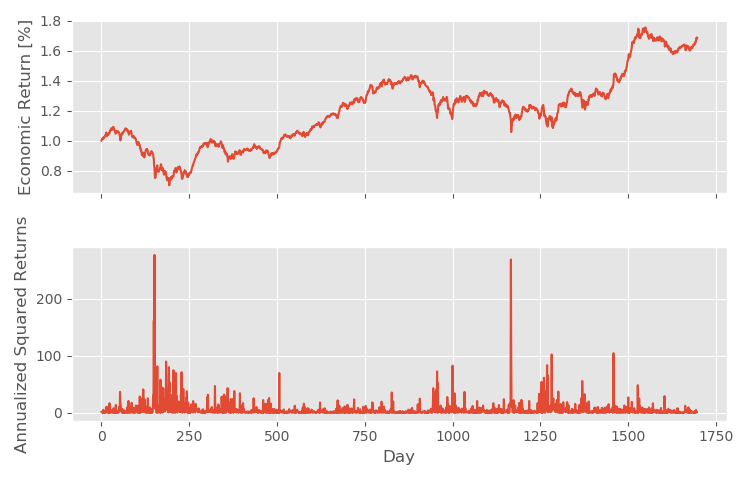
\includegraphics[scale = 0.7]{Plot/MarketReturn.png}
    \caption{Economic Return of the Market Portfolio}
    \label{MarketReturn}
\end{figure}

In Table \ref{DesStat} we present the descriptive statistics of the daily economic return distribution of the market portfolio. We observe that the market portfolio has a positive daily expected return of $0.04\%$. The data exhibits positive excess kurtosis, suggesting that our return distribution is a leptokurtic density. A leptokurtic density is one that has higher peak than a normal density. More peak means that a distribution also has fatter tails. Consequently, the probability of extreme outcomes is greater, compared to a normal distribution. Moreover, the negative skew indicates that the right tail has more probability density than the left tail. As a result, the mean is being skewed to the left of the center of the data. This is verified in Figure \ref{PercentilePlot} and Figure \ref{QQPlot}, as we observe that the economic return distribution is closely related, but not equal to a normal distribution.  

\begin{figure}
\centering
\begin{minipage}{.5\textwidth}
  \centering
  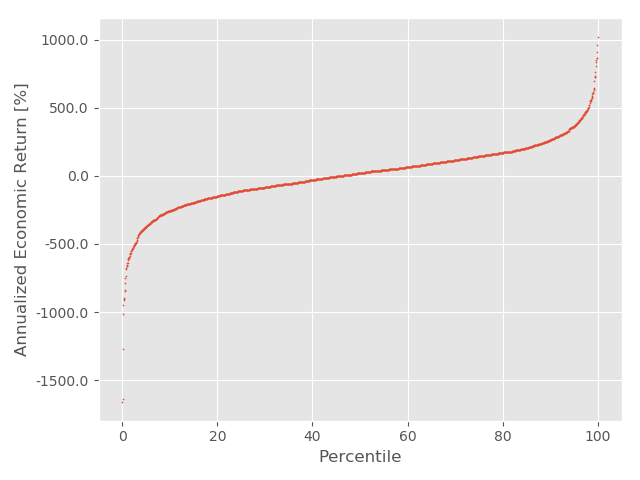
\includegraphics[scale=0.5]{Plot/PercentilePlot.png}
  \captionof{figure}{Percentile Plot of the Market Portfolio}
  \label{PercentilePlot}
\end{minipage}%
\begin{minipage}{.5\textwidth}
  \centering
  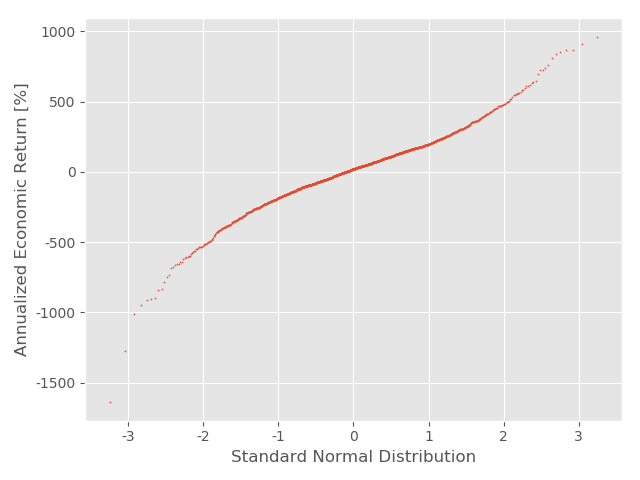
\includegraphics[scale=0.5]{Plot/QQPlot.png}
  \captionof{figure}{QQ Plot of the Market Portfolio}
  \label{QQPlot}
\end{minipage}
\end{figure}
\newcolumntype{P}[1]{>{\centering\arraybackslash}p{#1}}
%\begin{landscape}
\begin{longtable}{P{1cm}P{1.5cm}P{1.5cm}P{2.2cm}P{1.6cm}P{1.8cm}P{1.8cm}P{1cm}P{1cm}} 
\caption{Descriptive Statistics of the Market Portfolio}
\label{DesStat}\\
\hline
\textbf{Obs} & \textbf{Min} & \textbf{Max}&$\boldsymbol{E[r_{economic}]}$&\textbf{Median} &$\boldsymbol{\sigma^2_{economic}}$ &$\boldsymbol{\sigma_{economic}}$ & \textbf{Skew} & \textbf{Kurt} \\
\hline
\endfirsthead
\multicolumn{9}{c}%
{\tablename\ \thetable\ -- \textit{Continued from previous page}} \\
\hline
\textbf{Max}&$\boldsymbol{E(r_{economic})}$&\textbf{Median} &$\boldsymbol{\sigma^2_{economic}}$ &$\boldsymbol{\sigma_{economic}}$ & \textbf{Skew} & \textbf{Kurt} \\
\hline
\endhead
\hline \multicolumn{9}{r}{\textit{Continued on next page}} \\
\endfoot
\hline
\endlastfoot
\input{Input/DescriptiveStatsTable.txt}
\end{longtable}
\chapter{Methodology}
\label{Methodology}

The sample period for the various models we employ is the 250 last daily data points. All calculations are performed every day for all [x] stocks over the whole period used as a rolling window. The period used as a rolling window goes from January 2011 to September 2017, containing about 1500 daily data points. Bear in mind that transaction costs are not incorporated throughout this paper. The methodology of this paper is structured with four main components. 

In the first part of the study we calculate the daily idiosyncratic volatility (IV) for each of the selected stocks by applying the Fama French regression.

Secondly, we pool the stocks into four equally sized, equally weighted portfolios by their constituents proportion of daily IV to daily volatility, which we denote as the daily IV percentage. The equally weighted portfolios are rebalanced daily.

Thirdly, we construct an ARMA-GARCH return forecasting model. We estimate the ARMA-GARCH parameters and construct the one-day-ahead out-of-sample forecasts. Then, we compare the model’s one-day-ahead forecast with the realized return to obtain the daily return forecasting error. This is assigned to its associated portfolio that day and used to revise the return forecasting model. 

Lastly, we revise the return forecasting performance of both the individual stocks and the equally sized, equally weighted portfolios by applying statistical and economical metrics of comparison.

\begin{figure}
\centering
  \centering
  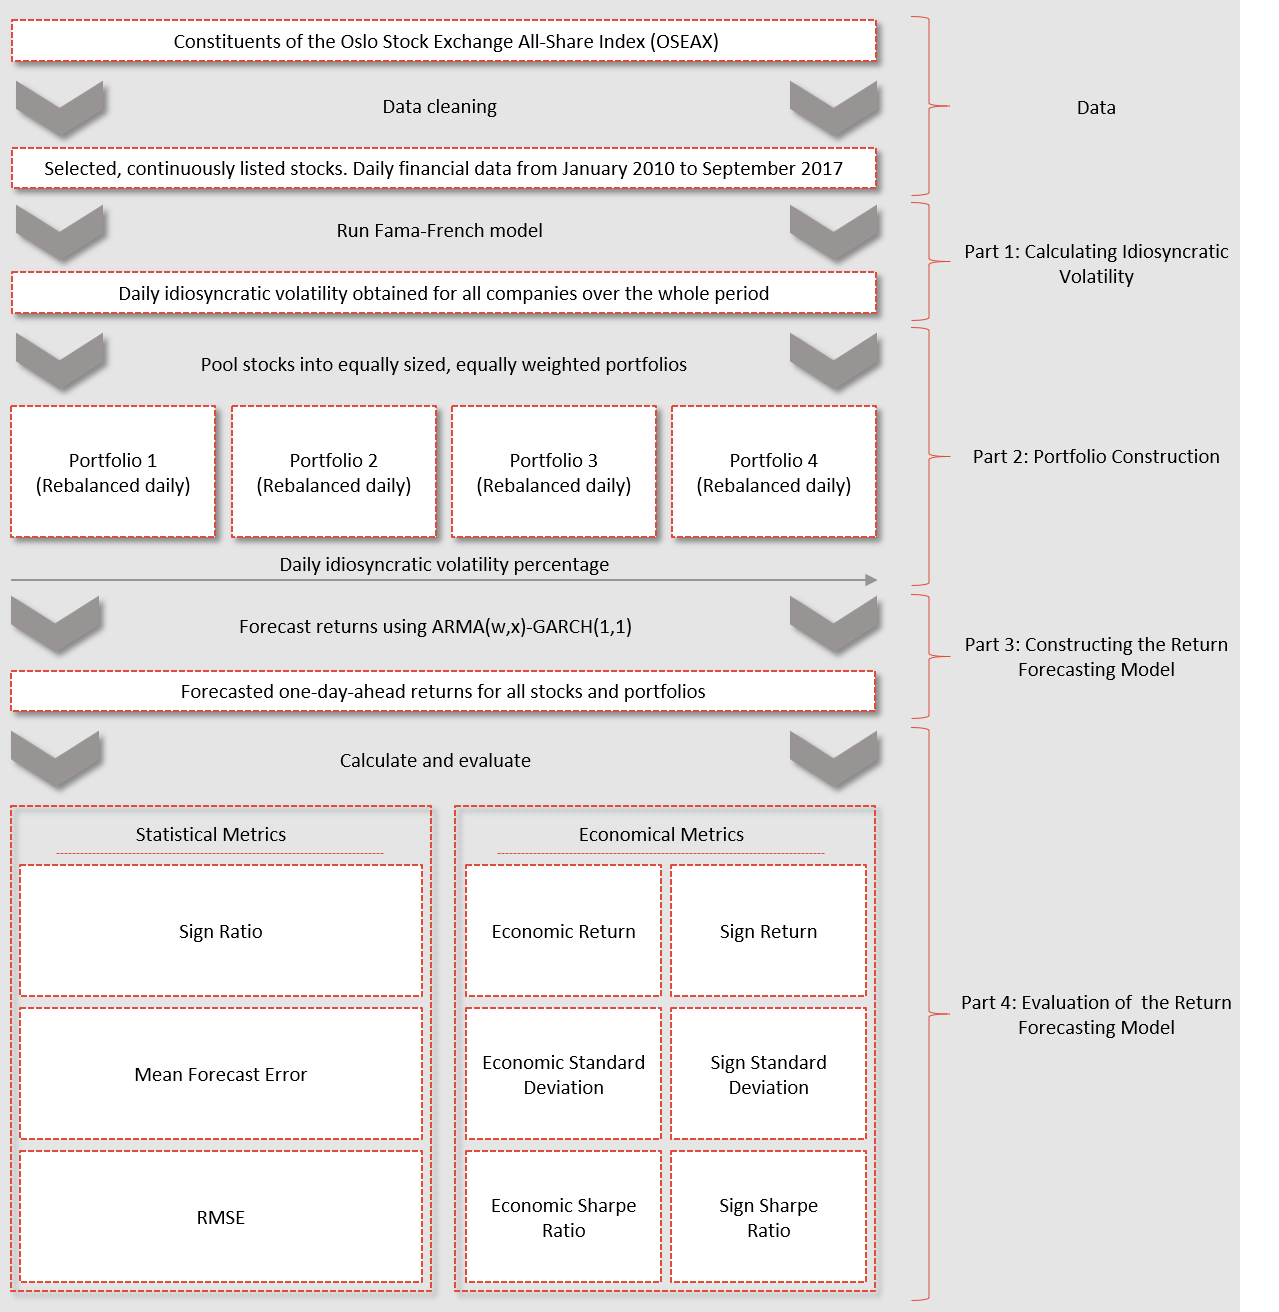
\includegraphics[scale=0.5]{Pictures/FlowChart.png}
  \captionof{figure}{Methodology: Flow Chart}
\end{figure}

\newpage
\section{Calculating the idiosyncratic volatility}

In this section, we describe how we implemented the Fama French three factor model, before we define idiosyncratic volatility.

\subsection{Implementation of the Fama French three factor model} The Fama French three factor model \cite{famafrench} incorporates the empirical fact that value and small-cap stocks have a tendency to outperform the market on a regular basis. Using their methodology we employ the following multiple linear regression:
\begin{align} 
    r_{i,t} - r_{f,t}= \alpha_{i,t} + \beta_{m,i,t}(r_{m,t} - r_{f,t}) + \beta_{SMB,i,t}r_{SMB,t} + \beta_{HML,i,t}r_{HML,t} + \epsilon_{i,t}, \quad  \forall i \in I \quad  \forall t \in T 
    \label{FFregression}
\end{align}

where $t$ indicates the day in the sample period, $r_{i,t}$ is the daily realized return of the stock $i$, $r_{f,t}$ is defined as the daily risk-free rate of Norwegian 10-years government bonds, $r_{m,t}$ is the daily return of the value-weighted market OSEAX portfolio, $r_{SMB,t}$ is the daily excess return of a portfolio consisting of small stocks relative to a portfolio consisting of big stocks, $r_{HML,t}$ is the daily excess return of a portfolio consisting of high book-to-market ratio stocks relative to low book-to-market stocks. $\beta_{m,i,t}$, $\beta_{SMB,i,t}$ and $\beta_{HML,i,t}$ are the corresponding coefficients resulting from the regression and the regression error is $\epsilon_{i,t}$.

More precisely, we define $r_{m,t}$, $r_{HML,t}$ and $r_{SMB,t}$ as:
\begin{align}
    r_{m,t} &= \sum_{i=1}^{N} r_{i,t} \cdot \frac{\text{MC}_{i,t}}{\sum_{s=1}^{N} MC_{s,t}},  \quad  \forall t \in T \\
    r_{SMB,t} &= \sum_{i=1}^{\frac{N}{2}} r_{i,t} \cdot \frac{\text{MC}_{i,t}}{\sum_{s=1}^{\frac{N}{2}} MC_{s,t}} - \sum_{k=\frac{N}{2}+1}^{N} r_{k,t} \cdot \frac{\text{MC}_{k,t}}{\sum_{s={\frac{N}{2}+1}}^{N} MC_{s,t}}, \quad  \forall t \in T \\
    r_{HML,t} &= \sum_{i=1}^{\frac{N}{2}} r_{i,t} \cdot \frac{\text{MC}_{i,t}}{\sum_{s=1}^{\frac{N}{2}} MC_{s,t}} - \sum_{k=\frac{N}{2}+1}^{N} r_{k,t} \cdot \frac{\text{MC}_{k,t}}{\sum_{s=\frac{N}{2}+1}^{N} MC_{s,t}} \quad  \forall t \in T
\end{align}
where $N$ is the number of stocks in the sample, $r_{i,t}$ and $MC_{i,t}$ is the realized return and market capitalization of stock $i$ at day $t$, respectively. 

\subsection{Definition of idiosyncratic volatility}
Consistent with Ang et al. \cite{angetal06} we define idiosyncratic volatility as the square root of the variance of the error term in the Fama French three factor model \cite{famafrench}. Hence, deriving from equation \ref{FFregression}, we have:
 \begin{align}
 IV_{i,t} &= \sqrt{Var[\epsilon_{i,t}]} \\
  &= \sqrt{Var[r_{i,t} - r_{f,t}- \alpha_{i,t}-\beta_{m,i,t}(r_{m,t} - r_{f,t}) - \beta_{SMB,i,t}r_{SMB,t} - \beta_{HML,i,t}r_{HML,t}]},  \quad  \forall i \in I \quad  \forall t \in T \\
 &= \sqrt{Var[r_{i,t}]+\beta_{1,i,t}^2Var[r_{m,t}]+\beta_{SMB,i,t}^2Var[r_{SMB,t}]+\beta_{HML,i,t}^2Var[r_{HML,t}]}, \quad  \forall i \in I \quad  \forall t \in T \\ 
 &= \sqrt{\sigma_{i,t}^2 - \beta^2_{m,i,t} \sigma_{m,t}^{2}- \beta^2_{SMB,i,t} \sigma_{SMB,t}^{2}- \beta^2_{HML,i,t} \sigma_{HML,t}^{2}}, \quad  \forall i \in I \quad  \forall t \in T
 \end{align}
where $t$ is the current day, T is the number of days the rolling window runs over and $IV_{i,t}$ is the IV of stock $i$ in day $t$. 

\section{Portfolio construction pooled by the constituents' daily IV percentage}
We have now described the methodology of estimating the daily IV percentage values. In this study, we seek to examine the relationship between the proportion of a stock's idiosyncratic volatility to volatility, the IV percentage. This because we find it interesting to examine stocks where the IV constitutes a large or small component of the stock's volatility, and not just in terms of magnitude. We define the daily IV percentage as the ratio:
\begin{align}
    \frac{IV_{i,t}}{\sigma_{i,t}}, \quad  \forall i \in I \quad  \forall t \in T
\end{align}

Further, we construct four equally sized, equally weighted portfolios by pooling stocks by their daily IV percentage. Portfolio 1 contains stocks with the lowest daily IV percentage, while portfolio 4 contains stocks with the lowest daily IV percentage. The portfolios are held for one day and the the equally-weighted return at the end of the current day is calculated. We rebalance the portfolios every day. 


\section{Constructing the return forecasting model: a dynamic ARMA($w,x$)-GARCH($1,1$)} 


\subsection{Theoretical background for the ARMA-GARCH return forecasting model}

Financial returns are often modelled as auto-regressive moving average (ARMA) time series with random disturbances having conditional heteroscedastic variances. The conditional mean and conditional variance will change at every point in time because it depends on the history of returns up to that point. That is, we account for the dynamic properties of returns by regarding their distribution at any point in time as being conditional on all the information up to that point. The distribution of a return at time t regards all the past returns up to and including time $t-1$ as being non-stochastic. We denote the information set, which is the set containing all the past returns up to and including time $t-1$, by $I_{t-1}$. The information set contains all the prices and returns that we can observe, like the filtration set in continuous time. 

We write $\sigma_t^2$ to denote the conditional variance at time $t$. This is the variance at time $t$, conditional on the information set. That is, we assume that everything in the information set is not random because we have an observation on it. When the conditional distributions of returns at every point in time are all normal we write:
\begin{align}
    r_t | I_{t-1} \sim N(0,{\sigma_t^2})
\end{align}

Often one would choose other distributions due to the fact that financial series often have fat tails. One option would be to use the Student-t distribution distribution or a skewed version of it. This paper assumes that returns are having a normal distribution. 

\subsubsection{The Conditional Mean Equation, ARMA($w$,$x$)}

For modeling data series we used two common concepts of conditional mean: the auto regressive (AR) process and the moving average (MA) process. Together the two processes constitute the conditional mean equation. 

The AR process is given by:
\begin{align}
    r_{i,t}=c_i + \sum_{j=1}^w\kappa_j r_{i,t-j} + \epsilon_{i,t},\quad \epsilon_{i,t} | I_{i,t-1} \sim N(0,{\sigma_{i,t}^2}) \label{ConditionalMeanEquation}
\end{align}
where $\kappa_j$ is the lag parameter of the observed variable, $r_t$ is the random observed variable at time $t$ dending on the previously realized values of $r_{t-j}$, $c$ is the mean constant and $\epsilon_t$ the white noise.

The MA process is given by:
\begin{align}
    r_{i,t}=c_i + \sum_{j=1}^x\mu_{i,j} \epsilon_{i,t-j} + \epsilon_{i,t},\quad \epsilon_{i,t} | I_{i,t-1} \sim N(0,{\sigma_{i,t}^2}) \label{ConditionalMeanEquation}
\end{align}
where $\mu_j$ is the lag parameter of the observed variable, $r_t$ is the random observed variable at time $t$ depending on the previously realized values of $\epsilon_{t-j}$, $c$ is the mean constant and $\epsilon_t$ the white noise.

The combination of both the AR-process and MA-process, gives us the ARMA process described by:
\begin{align}
    r_{i,t}=c_i+\sum_{j=1}^w\kappa_{i,j} r_{i,t-j}+\sum_{j=1}^x\mu_{i,j} \epsilon_{i,t-j}+\epsilon_{i,t},\quad \epsilon_{i,t} | I_{i,t-1} \sim N(0,{\sigma_{i,t}^2}) \label{ConditionalMeanEquation}
\end{align}

\subsubsection{The Conditional Variance Equation, GARCH($y,z$)}
As financial data time series usually exhibit volatility clustering, a model dealing with
conditional heteroskedasticity should be considered. We use the GARCH model introduced by (Bollerslev, 1986),which is a generalization of the ARCH model that was originally developed by (Engle, 1982). The ARCH model allows for long lags in conditional variance and the GARCH model extends it in the way that it allows for both long lags in conditional variance and a more flexible lag structure.

The GARCH($y$,$z$) has the conditional volatility equation given by:

\begin{align}
    \sigma_{i,t^2} &= \omega_i + \sum_{j=1}^y\alpha_{i,j}\epsilon_{i,t-j}^2+\sum_{j=1}^z\beta_{i,j}\sigma_{i,t-j}^2,\quad\epsilon_{i,t} | I_{i,t-1} \sim N(0,{\sigma_{i,t}^2}) \label{ConditionalVolatilityEquation}
\end{align}

The GARCH error parameter $\alpha$ measures the reaction of conditional volatility to market shocks. When $\alpha$ is relatively large, above 0.1, the volatility is very sensitive to market events.

The GARCH lag parameter $\beta$ measures the persistence in conditional volatility irrespective of anything happening in the market. When $\beta$ is relatively large, above 0.9, then volatility takes a long time to die out.

\subsubsection{Long term volatility}

In the absence of market shocks the GARCH variance will eventually settle down to a steady state value. This is the value $\bar{\sigma}^2$ such that ${\sigma_t^2} = \bar{\sigma}^2$ for all t. We call $\bar{\sigma}^2$ the unconditional variance of the GARCH model. It corresponds to a long term average value of the conditional variance. The theoretical value of the GARCH long term or unconditional variance is not the same as the unconditional variance in a moving average volatility model. The moving average unconditional variance is called the i.i.d. variance because it is based on the i.i.d. returns assumption. The theoretical value of the unconditional variance in a GARCH model is clearly not based on the i.i.d. returns assumption. In fact, the GARCH unconditional variance differs depending on the GARCH model. The long term or unconditional variance is found by substituting ${\sigma_t^2} = {\sigma_{t-1}^2} = \bar{\sigma}^2$ into the GARCH conditional variance equation.We also use the fact that $E(\epsilon_{t-1}^2)=\sigma_{t-1}^2$. This yields the following formula for the long term variance of the GARCH model:

\begin{align}
    \bar{\sigma}_i^2=\frac{\omega_i}{1-(\sum_{j=1}^y\alpha_{i,j}+\sum_{j=1}^z\beta_{i,j})} \label{longTermVolatilityGARCH}
\end{align}

\subsubsection{Parameter Estimation}

The plain vanilla ARMA and ARMA-GARCH parameters are estimated by maximizing the value of the log likelihood function. As mentioned earlier, in this paper we assume that the distribution of the error process is normal with expectation 0 and conditional variance ${\sigma_t^2}$. Furthermore, we have assumed stationarity, so the unconditional variance, in the case of plain vanilla ARMA, is ${\bar\sigma^2}$. With these assumptions in mind, we can use the normal log likelihood function.

\subsubsection{Plain Vanilla ARMA($w,x$)}

Maximizing the ARMA likelihood reduces to the problem of maximizing:
\begin{align} 
    ln(L_{i,t})=-\frac{1}{2}\sum_{t=1}^T\bigg( ln(\sigma_{i}^2)+(\frac{\epsilon_{i,t}}{\sigma_i})^2\bigg)  \label{MaximumLikeARMA}
\end{align}
with respect to all the parameters. To do this we solve the conditional mean equation (\ref{ConditionalMeanEquationARMA}) for $\epsilon_t$:
\begin{align}
     \epsilon_{i,t}=r_{i,t}-\sum_{j=1}^w\kappa_{i,j} r_{i,t-j}-\sum_{j=1}^x\mu_{i,j} \epsilon_{i,t-j}-c_i \label{ConditionalMeanEquationOnEpsilon}
\end{align}
Finally we insert the above equation (\ref{ConditionalMeanEquationOnEpsilonARMA}) and the conditional volatility equation (\ref{ConditionalVolatilityEquation}) into the maximum likelihood function (\ref{MaximumLikeARMA}):
\begin{align} 
    ln(L_{i,t})=-\frac{1}{2}\sum_{t=1}^T\Bigg( ln(\sigma_i^2)+\Big(\frac{(r_{i,t}-\sum_{j=1}^w\kappa_{i,j} r_{i,t-j}-\sum_{j=1}^x\mu_{i,j} \epsilon_{i,t-j}-c_i)^2}{\sigma_i^2}\Big)\Bigg)  \label{fullMaximumLikeARMA}
\end{align}

\subsubsection{ARMA($w,x$)-GARCH($y,z$)}
Maximizing the ARMA-GARCH likelihood reduces to the problem of maximizing:
\begin{align} 
    ln(L_{i,t})=-\frac{1}{2}\sum_{t=1}^T\bigg( ln(\sigma_{i,t}^2)+(\frac{\epsilon_{i,t}}{\sigma_{i,t}})^2\bigg)   \label{MaximumLike}
\end{align}
with respect to all the parameters. The conditional mean equation is solved on epsilon, just as in equation \ref{ConditionalMeanEquationOnEpsilon}. The equation is then inserted, together with the conditional volatility equation (\ref{ConditionalVolatilityEquation}), into the maximum likelihood function (\ref{MaximumLike}):
\begin{align} 
    ln(L_{i,t})=-\frac{1}{2}\sum_{t=1}^T \Bigg(ln\Big(\omega_i + \sum_{j=1}^y\alpha_{i,j}\epsilon_{i,t-j}^2+\sum_{j=1}^z\beta_{i,j}\sigma_{i,t-j}^2\big)+\Big(\frac{(r_{i,t}-\sum_{j=1}^w\kappa_{i,j} r_{i,t-j}-\sum_{j=1}^x\mu_{i,j} \epsilon_{i,t-j}-c_i)^2}{\omega_i + \sum_{j=1}^y \alpha_{i,j} \epsilon_{i,t-j}^2 +\sum_{j=1}^z\beta_{i,j}\sigma_{i,t-j}^2}\Big)\Bigg)   \label{fullMaximumLike}
\end{align}
The parameter constraints are:
\begin{align} 
    \omega_i>0,\quad\quad \alpha_{i,j},\beta_{i,j}\geq0 \quad \forall j, \quad \sum_{j=1}^y\alpha_{i,j}+\sum_{j=1}^z\beta_{i,j}<1 \label{ParameterConstraints}
\end{align}

\subsection{Implementation of the dynamic ARMA($w,x$)-GARCH($1,1$)}
To forecast returns we will try to fit an auto regressive moving average return model (ARMA) of order ($w,x$) with asymmetric generalized auto-regressive conditional hetereoscadasticity (GARCH) of order ($1$,$1$). The estimation of the ARMA($w,x$)-GARCH($1,1$) parameters is done in R, while the rest of the calculations in this paper is done in Python. The reason we chose to calculate the parameters of the ARMA($w,x$)-GARCH($1,1$) in R, is because there are currently no packages in Python supporting ARMA-GARCH, only AR-GARCH. 

The first thing to be decided, is the ARMA order. In other words, we have to decide which values the parameters, $w$ and $x$, in the conditional mean equation (\ref{ConditionalMeanEquation}) should have. The parameters and hence the maximum likelihood is calculated for all combinations of $w$ and $x$, using equation \ref{fullMaximumLikeARMA}, where $w\in[0,3]$ and $x\in[0,3]$. The final values of $w$ and $x$, the ARMA order, to use in our forecast is chosen based on the the Akaike information criterion (AIC). AIC is an estimator of the relative quality of statistical models for a given set of data. Given a collection of models for the data, AIC estimates the quality of each model, relative to each of the other models. Thus, AIC provides a means for model selection. The AIC of a given model is calculated using the following equation:
\begin{align}
    AIC_{i,t}=2k_i-2ln(L_{i,t})
\end{align}
where $k$ is the number of estmated parameters and $L$ is the maximum value of the likelihood function. 

After the decision is made of which ARMA order to use, equation (\ref{fullMaximumLike}) is solved. There is no guarantee that the maximum likelihood of the ARMA-GARCH will converge. To increase the probability of convergence, the algorithm in R tries four different solvers. If there is no convergence, the conditional mean parameters are found using plain vanilla ARMA (\ref{fullMaximumLikeARMA}) and not ARMA-GARCH (\ref{fullMaximumLike}). The maximum likelihood function of plain vanilla ARMA will almost always converge because it is linear. If the plain vanilla ARMA does not converge, the process above is repeated with the ARMA order giving second best AIC, and so on, until convergence is achieved.

The ARMA($w,x$)-GARCH($1,1$) parameters are estimated based on the information set for each stock, $i$, for every time step, over the whole period used as a rolling window. The time step is one-day-ahead and the information set, sample, which the parameters are estimated from are the past 250 daily returns. As mentioned in the introduction to this chapter, there are [x] stocks, the period used as a rolling window is from January 2011 to September 2017, constituting about 1500 trading days. The model setup results in a huge number of needed calculations, and as a consequence, we were granted access to the calculation cluster Solstorm belonging to the Department of Industrial Economics and Technology Management at NTNU. 

One may argue that a information set bigger than 250 should be used, as the standard errors of the parameters are only valid asymptotically. This, additional return forecasting model spesification and other return forecasting models are further discussed in Chapter \ref{FutureWork}.


\subsection{Return forecasting}

After the model in the previous subsection is run on the data, we obtain optimal values for all the parameters for each stock every day. To forecast the the one-day-ahead return, and hence test our out-of sample performance, we need to compute the conditional expected return of the conditional mean equation (\ref{ConditionalMeanEquation}). The expected return at time $t$ for a given stock, $i$, is:
\begin{align} 
    E(r_{i,t})=c_i+\sum_{j=1}^w\kappa_{i,j} r_{i,t-j}+\sum_{j=1}^w\mu_{i,j} \epsilon_{i,t-j} \label{ExpectedConditionalMean}
\end{align}
The expectation of the error process, $\epsilon_t$, is assumed to be zero. The parameters obtained in the previous subsection is our best guess on what the parameters would be tomorrow. Hence, the optimal parameters at time $t$ is used to forecast the return at time $t+1$. Using equation \label{ExpectedConditionalMean}, our forecast at time $t$ for time $t+1$ for a given stock,$i$, is:
\begin{align} 
    E(r_{i,t+1})=c_i+\sum_{j=0}^w\kappa_{i,j} r_{i,t-j}+\sum_{j=0}^x\mu_{i,j} \epsilon_{i,t-j}
\end{align}

\section{Evaluation of the return forecasting model performance}
In the last section we specified the return forecasting model, we now wish to evaluate the model's return forecasting performance in terms of both statistical and economical metrics. 

\subsection{Statistical Metrics}

The return forecasting model produces a series of return forecasting estimates, we calculate the return forecasting error for each day in the out-of-sample period. We define the return forecasting error as:
\begin{align}
    \epsilon_{i,t}^{f} = r_{i,t}^{r} - r_{i,t}^{e}
\end{align}
where $\epsilon_{i,t}^{f}$ is the return forecasting error, the difference between the return forecasting estimate, $r_{i,t}^{e}$, and realized returns, $r_{i,t}^{r}$, for all stocks and all time steps.

In order to assess the return forecasting accuracy and precision, we define two statistical metrics.

Firstly, as a statistical measure of accuracy, we define the mean forecast error, that is the \textbf{bla bla bla}, as:

\textbf{Fyll inn matematisk formel}

Secondly, as a statistical measure of precision, we define the root mean square error metric (RMSE), that is the standard deviation of the residuals, as:
\begin{align}
    RMSE_{\tau} = \sqrt{\frac{\sum_{i=1}^{N}(r_{i,t}^{r} - r_{i,t}^{e})^{2}}{n}}, \quad \forall \tau in \Sigma
\end{align}
where $i$ is stock and $\tau$ is the current period and $\Sigma$ is the total number of periods. We calculate the RMSE for each portfolio and each period, summing the total RMSE for each portfolio over the total sample period, before finding the average by dividing by number for periods:
\begin{align}
    RMSE_{b} = \frac{1}{|\Sigma|}\sum_{\tau=1}^{|\Sigma|}\sqrt{\frac{\sum_{i=1}^{N}(r_{i,t}^{r} - r_{i,t}^{e})^{2}}{n}}, \quad \forall b \in B
\end{align}

Another statistical metric, as a measure of the market timing ability of the return forecasting model, we calculate the proportion of times the model correctly predicted the direction of the return. We define this percentage as Sign and its corresponding return as $r_{sign}$. 

\subsection{Economical Metrics}

Moreover, we also wish to apply economical metrics. 

We define the economic return, $r_{economic}$, as the annualized return obtained from following a buy-and-hold strategy, holding a stock from the start until the end of the period.

Furthermore, we wish to examine the profitability of following the predictions of our return forecasting model, compared to an ordinary buy-and-hold strategy. 

Hence, we define the sign return as following the one-day-ahead predictions from the return forecasting model from the start to the end of the period used as a rolling window. That means taking a long position if the model predicts a positive return, and a short position if the model predicts a negative return for the next day. The annualized return of this strategy is defined as the sign return, $r_{sign}$. If the prediction is correct, the realized return is assigned to the $r_{sign}$. Likewise, if the prediction is wrong, the realized return is withdrawn from the accumulated return, $r_{sign}$.

In addition, we calculate standard deviations of the economic and sign return. We define alpha, $\alpha$, as the difference $r_{sign}-r_{economic}$. This is the excess return from following the sign strategy compared to the buy-and-hold strategy. 

Finally, we find the Sharpe ratio of the annualized economic return and annualized sign return, respectively. The Sharpe ratio is defined as the excess return over the risk free rate, divided by the standard deviation.

The result section will usually be tabulated or graphed, and each table or figure should be described, noting any interesting features – whether expected or unexpected, and in particular, inferences should relate to the original aims and objectives of the research outlined in the introduction. Results should be discussed and analysed, not simply presented blandly. Comparisons should also be drawn with the results or similar existing studies if relevant – do your results confirm or contradict those of previous research? Each table or figure should be mentioned explicitly in the text. Do not include in the project any tables or figures which are not discussed in the text. It is also worth trying to present the results in as interesting and varied way as possible – for example, including figures and charts as well as just tables.


\chapter{Results}

\textbf{DUMMY TEXT}
The in-sample and out-of-sample forecasting ability of the different linear and nonlinear models described above were assessed in terms of statistical accuracy and economic criteria. The analysis was based on one-step-ahead forecasting. Once each model had been estimated, we constructed the in-sample and out-of-sample forecasts without updating the parameters of the model that were
obtained from the training set.

Table I shows the results of the goodness of forecasts for the different models and time periods and
for the corresponding forecast horizons. The main conclusions are two.


\begin{figure}
    \centering
    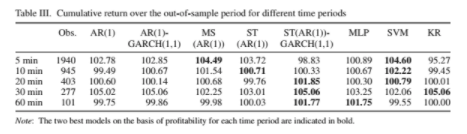
\includegraphics{Pictures/cumret.png}
    \caption{Example table of cumulative return}
    \label{fig:my_label}
\end{figure}

\begin{figure}
    \centering
    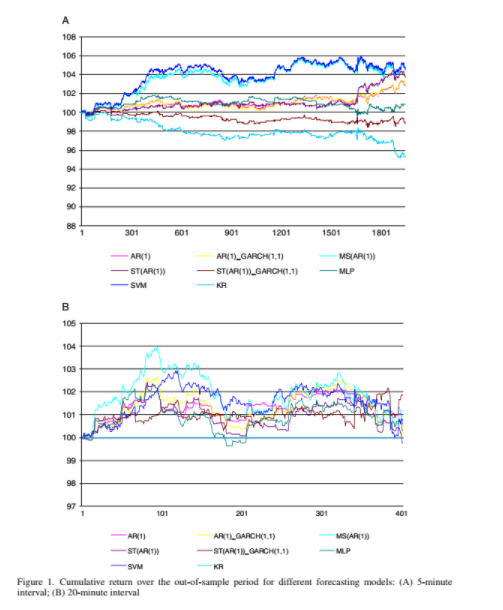
\includegraphics{Pictures/cumretGraphs.png}
    \caption{Example graphs of cumulative return}
    \label{fig:my_label}
\end{figure}




\begin{longtable}{|c|c||c|c||c|c||c|} 
\caption{Forecast Stocks}
\label{Forecast Stocks}\\
\hline
\textbf{1} & \textbf{2} & \textbf{3} & \textbf{4} & \textbf{5} & \textbf{6}& \textbf{7} \\
\hline
\endfirsthead
\multicolumn{7}{c}%
{\tablename\ \thetable\ -- \textit{Continued from previous page}} \\
\hline
\textbf{1} & \textbf{2} & \textbf{3} & \textbf{4} & \textbf{5} & \textbf{6}& \textbf{7} \\
\hline
\endhead
\hline \multicolumn{7}{r}{\textit{Continued on next page}} \\
\endfoot
\hline
\endlastfoot
\input{Input/ForecastsStocks.txt}
\end{longtable}

\chapter{Conclusions}

We performed an extensive evaluation of the relationship between the daily IV percentage and the out-of-sample one-day-ahead forecasting performance of ARMA-GARCH. The same conclusion is derived from the evaluation of both individual stocks and portfolios created by pooling stocks according to their daily IV percentage. 

Firstly, using daily closing prices, from January 2010 to September 2017, for all the constituents of the Oslo Stock Exchange All-Share Index (OSEAX), we have showed that the one-day-ahead return of stocks and portfolios with higher daily IV percentage is more difficult to forecast in terms of magnitude and direction than stocks and portfolios with lower daily IV percentage. In other words, we found a negative relationship between daily IV percentage and forecast performance in terms of magnitude and direction. 

Secondly, we have shown that the forecasting performance of the ARMA-GARCH is good. Trading according to the forecasting model generates returns better than those obtained by following a simple buy-and-hold strategy, across all levels of daily IV percentage. 

Finally, as the  daily IV percentage of stocks and portfolios increases, the excess return generated from trading according to the forecast model compared to the buy and hold-strategy increases. The positive relationship between daily IV percentage and return generated from the forecast model, despite the negative relationship between daily IV percentage and forecast performance in terms of magnitude and direction, may be seen contradictory. However, we have shown that stocks and portfolios with higher daily IV percentage also tend to have higher economic standard deviation. As a result, it might be easier for the forecasting model to predict the bigger directional movements when economic standard deviation, and hence daily IV percentage, is greater. 
A list of references (a list of all papers, books or web pages referred to in the study, irrespective of whether you read them, or found them cited in other studies), as opposed to bibliography (a list of items that you read, irrespective of whether you referred to them in the study) is usually required.

\chapter{References}
% Include more chapters as required.
%%=========================================
\appendix
%This is Appendix A - Acronyms
%%=========================================

\chapter{Acronyms}
\begin{description}
\item [CAPM]
\item[FTA] Fault tree analysis
\item[MTTF] Mean time to failure
\item[RAMS] Reliability, availability, maintainability, and safety
\end{description}
\chapter{Additional Information}

% Include more appendices as required.
%%=========================================
\bibliographystyle{apa}
\addcontentsline{toc}{chapter}{\bibname}
\bibliography{refs}  
%%=========================================


\end{document}
